\documentclass[a4paper, 12pt]{article}

\usepackage{setspace}
\doublespacing

%% Language and font encodings
\usepackage[english]{babel}
\usepackage[utf8x]{inputenc}
\usepackage[T1]{fontenc}

%% Sets page size and margins
\usepackage[a4paper,top=3cm,bottom=2cm,left=3cm,right=3cm,marginparwidth=1.75cm]{geometry}

%% Useful packages
\usepackage{amsmath}
\usepackage{graphicx}
\usepackage{apacite}
\usepackage{indentfirst}

\title{Novel Object Recognition Task for Memory Analysis in Rats}
\author{Andy Malinsky}

\begin{document}
\maketitle

\section{Introduction}
Memory is one of the most essential factors to survival. Further understanding how it works is the foundational idea of this study. Humans, for example, are a species that thrives on predicting future events in order to minimize potential threat levels. To do so, however, requires some form of previously stored knowledge or, in other words, memory. Novel Object Recognition (NOR) is one way of assessing learned memory, where any impairments negatively affect performance \cite{broadbent2004spatial}. 

Previous studies involved the use of rodents in controlled laboratory conditions along with distinct objects for testing. One object is presented at first. Then a novel object is presented, and the behavior of the rodents should illustrate a learned response. As a measurement for object recognition, the absolute difference in exploration time of novel and familiar objects may be implemented \cite{leger2013object, antunes2012novel}. This procedure exploits the rodent's innate curiosity towards novel objects \cite{bevins2006object}. This may be mostly in part that the subject is constantly searching for new sources for food.

Anticipated results state that time spent with the novel object should be greater than time spent with the familiar object, serving as a replication study to ensure expected results found by previous work \cite{leger2013object, reger2009ontogeny, sutcliffe2007influence}. By analyzing behavior in rodents, we seek to discover that more time will be spent with novel objects, thereby providing more evidence of the formation of learned memory.

\section{Methods}
\subsection{Subjects}
For the present study, we used 16 Male and Female Sprague-Dawley rodents to evaluate memory in the NOR task. The provided light cycle consisted of 12 hours of light and dark respectively. They were allowed continuous access to food and water. Their weight ranged from 350-450 grams. They were housed in the Boyer Hall rat vivarium.

\subsection{Apparatus}
The materials used were of crucial importance for achieving ideal conditions. We utilized a roughly square grey polyethylene container.. The box has no lid and has dimensions of 22.5 X 24 X 13.5 in (l X w X h). The walls should be tall enough to not allow the subject to escape. The floor of the container was divided into four equal quadrants. For the objects, two small plastic bowls were used. One was blue and one was green. Both were similar in size and shape. It is important to select objects that are different enough to be distinguishable, but also similar in complexity to avoid bias. We also, employed a white noise machine during manipulation. A special cleaning spray was used to remove excess dander or scents. Testing was conducted in an isolated and enclosed room.

\subsection{Procedure}
A strict procedure needs to be  maintained to ensure balanced results across subjects. Habituate to testing room and box for 10 minutes each. On training day, place two identical objects on the same diagonal in the apparatus (opposite quadrants). Record the amount of time spent in each quadrant containing an object. The subject is expected to spend an equal amount of time investigating each object.

On testing day, place one familiar object from training and one novel object on the same diagonal as training day. Record the amount of time spent in each quadrant containing an object. The subject is expected to spend more time investigating the novel object.
For each step, place the subject in the middle of the apparatus. Clean the apparatus and objects between each step.

\subsection{Statistical Analysis}
We utilized various statistical measurements to infer conclusions from gathered results. We employ an Independent Samples T-test, where we calculate mean and standard deviation of time spent with the novel object.

\section{Results}
The figure below represents our results for the NOR task across two days.

\begin{figure}[h!]
    \centering{}
    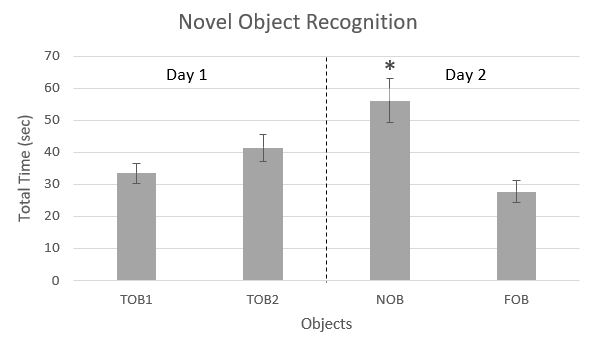
\includegraphics{norChart.JPG}
    \caption{TOB1 and TOB2 represents Training Object 1 and Training Object 2 respectively. NOB represents the novel object. FOB represents the familiar object. * indicates that NOB is significantly significant from FOB.}
    \label{fig:norChart}
\end{figure}

On training day, there was no significant difference in time spent with OB1(M = 33.5) and OB2(M = 41.4) (T(12) = -2.077, p = .060). On testing day, there was a significant difference in time spent with NOB(M = 56) and FOB(M = 27) (T(12) = 3.370, p = .006). See Figure \ref{fig:norChart} for more details.

\section{Discussion}
In the current study, the presentation of the novel object versus a familiar object resulted a significant difference in average investigation time. The gathered results demonstrated that the subjects spent more time with the novel object than with the familiar object. This result supports the original hypothesis of this study in relation to the expected results established in prior studies. Other studies \cite{reger2009ontogeny, anderson2004effects} found similar results, but with differences in age across control groups being another factor. Other factors such as gender were explored by \cite{sutcliffe2007influence}, yielding comparable findings in the NOR task, but with separate male and female groups. Other factors such as initial habituation time were considered \cite{leger2013object}, in order to find variation in investigation time toward the novel object.

This study, however, has some limitations. Inconsistency in exploratory activity caused from the openness or elevation of the apparatus or mild food deprivation could lead to an irrelevancy in differences between objects \cite{antunes2012novel}. Also, it assumed that every subject has a functional memory. Potential memory deficits that may stem from certain biological conditions would negatively effect a subject's ability to distinguish a novel object from a familiar one \cite{bevins2006object}.

Possible future directions for experimentation could be to explore potential transfer learning effects or number of iterations for individual rats. Would there be a difference in investigation time between a group of rats learning from scratch and a group of rats who have undergone a whole NOR study already? This would investigate transfer effects, as the rats with prior experience may show signs of expectations that would otherwise not be present in the rats training with no prior knowledge. Also, would the number of iterations in swapping novel and familiar objects have any effects on investigation time? For example, an iteration could be considered as the pipeline of starting with two objects until familiarity, replacing one with a novel object, then eventually replacing the other previously familiarized object with another copy of the same novel object, thus ending with two familiar objects again. Each iteration would present another novel object for exploration. The question of whether or not exploration time would significantly change over time would be proposed.

This results from this study displayed the significance of memory and the role it plays in our lives. Using the Novel Object Recognition task as a tool for measuring learned memory behavior helped support the expected findings, and may be a potentially useful tool for future studies investigating our understanding of memory.

% APA References
\bibliographystyle{apacite}
\bibliography{bib.bib}

\end{document}